\subsection{Signals & Systems}

We've attempted throughout the writing of all these lecture notes to properly explain the things we need. This topic is an exception. 

In this section, we'll cover some basic ideas of a broad field called Linear Systems, or "Signals and System". Covering this topic in exhaustive manner is way beyond the scope of this lecture notes, though we need some knowledge about linear systems to understand properties of some of the circuits we will study. I will not spend too much time explaining this in an easy way, but rather assume that you already understand the basic principles and that this will serve as a reminder or reference. If you do not understand the concepts, there is no better resource than the classic textbook on the topic by Alan V. Oppenheim  "Signals and Systems" \footnote{Here is a link to the PDF version: \url{https://eee.guc.edu.eg/Courses/Communications/COMM401\%20Signal\%20&\%20System\%20Theory/Alan\%20V.\%20Oppenheim,\%20Alan\%20S.\%20Willsky,\%20with\%20S.\%20Hamid-Signals\%20and\%20Systems-Prentice\%20Hall\%20(1996).pdf}}. I would never manage to quickly explain things better than it already is in this textbook, so if you're confused about anything that I am presenting here, save yourself some precious time and go have a look at the textbook! The topic is very well introduced to the precision we need in the textbook, so I will simply \textbf{shamelessly} copy paste the content here for convenience. Let's start.

\subsubsection{Linear-Shift-Invariant System}

\begin{figure}[H]
    \centering
    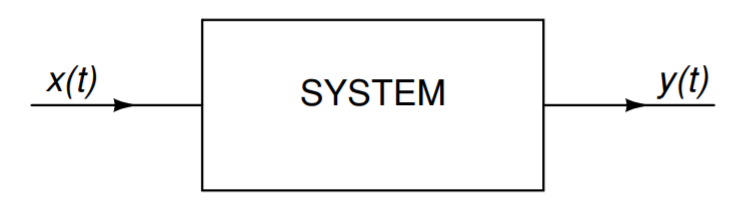
\includegraphics[width=0.5\linewidth]{../../Figures/Linear_Systems.PNG}
    \caption{Typical black-box representation of a linear system. Its input is the signal $x(t)$ and its output is the signal $y(t)$. Adapted from textbook}
    \label{fig:Linear_Systems_Black_Box}
\end{figure}

In linear systems theory, a system is treated as a black box that does not reveal its internal states, and is characterized only by the relationship between its input and output (see Figure \ref{fig:Linear_Systems_Black_Box}). If a system has no internal stored energy, then its output response $y(t)$ is forced entirely by the input $x(t)$:

\begin{equation}
    y(t) = F [x(t)] \textrm{, where F is the transfer function} 
\end{equation}

\textbf{Conditions for Linearity:}

A system is said to be linear if it obeys the two fundamental principles of homogeneity and additivity (see Figure \ref{fig:Linear_Systems_Properties}). 

\begin{itemize}
    \item Additivity: The principle of additivity states that if the input signal is composed
of elementary signals, then the system’s response is the composition of its
responses to each of the elementary signals:
    \begin{equation}
        F[x_1(t) + x_2(t) + ... + x_n(t)] = F[x_1(t)] + F[x_2(t)] + ... + F[x_n(t)]
    \end{equation}
    \item Homogeneity: The principle of homogeneity states that output scales linearly with the
input:
    \begin{equation}
        F[\alpha x(t)] = \alpha F[x(t)] 
    \end{equation}
\end{itemize}

\begin{figure}[H]
    \centering
    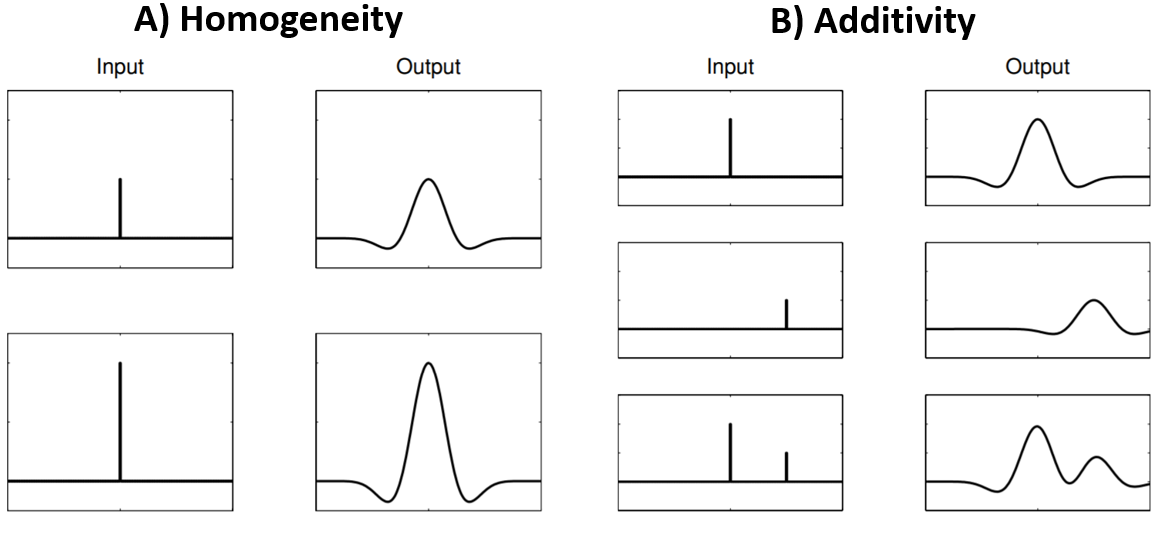
\includegraphics[width=0.9\linewidth]{../../Figures/Linear_Systems_Properties.PNG}
    \caption{Fundamental principles of linear systems. Adapted from textbook}
    \label{fig:Linear_Systems_Properties}
\end{figure}

\textbf{Time and Shift invariance}


This is another useful property of many systems. A system is said to be shift-invariant if its responses to identical stimuli shifted in time are also identical, except for the corresponding
time shift. Given input signal $x(t)$., its time-shifted variant $x(t-\tau)$ will produce:
\begin{equation}
    F[x(t-\tau)] = y(t-\tau)
\end{equation}

Time invariance and linearity are two independent characteristics. Not all
linear systems are time-invariant and, similarly, not all time-invariant systems
are linear

\begin{figure}[H]
    \centering
    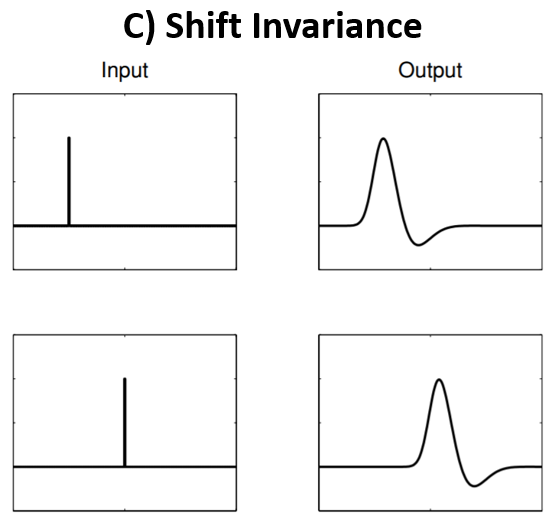
\includegraphics[width=0.5\linewidth]{../../Figures/Shift_Invariance.PNG}
    \caption{Shift Invariance Property. Adapted from textbook}
    \label{fig:Shift_Invariance}
\end{figure}

\subsubsection{Convolution}

Please do yourself a favour and do not even hope to understand convolution through this explanation. Go have a look at the Oppenheim textbook I mentionned earlier, it's a very complicated idea to understand and needs time. Though I must say you barely need to understand this for the exam. 

Convolution is an important mathematical operator used in linear systems analysis. The convolution of two time-varying signals, $v(t)$ and $w(t)$, is:

\begin{equation}
    x(t) \circledast h(t) &= \int_{- \infty}^{\infty} {v(\lambda w(t-\lambda)} d\lambda
\end{equation}


where $\lambda$ is the integration variable, and $t$ is the independent variable

\subsubsection{Impulses}

The \textit{unit impulse} or \textit{Dirac delta function} $\delta (t)$is not a function in the strict mathematical sense. It is defined by a set of assignment rules. 
\begin{itemize}
    \item If $v(t)$ is a continuous function at $t=0$, then:
    \begin{equation}
        \int_{t_1}^{t_2} {v(t)\delta (t)} dt = \left\{
    \begin{array}{ll}
        \ v(0) & \mbox{if } \{t_1<0<t_2\} \\
        \ 1 & \mbox{Otherwise}
    \end{array}
\right.
    \end{equation}
    \item If $\epsilon$ is an arbitrary small number
    \begin{equation}
        \int_{-\infty}^{\infty} {\delta (t)} dt = \int_{-\epsilon}^{\epsilon} {\delta (t)} dt = 1
    \end{equation}
\end{itemize}

From these rules we can infer that $\delta (t)$ has unit area at $t = 0$ and that $\delta(t) = 0$, for all $t \neq 0$. We can also note that the Dirac delta function has no mathematical or physical meaning, unless it appears under the integral operator.

\subsubsection{Impulse Integration properties}

When used in conjunction with the integral operator, the Dirac delta function
has the following properties:

\begin{itemize}
    \item Replication:
        \begin{equation}
             v(t) \circledast \delta (t- \tau) = v(t - \tau)
        \end{equation}
        
    \item Sampling:
        \begin{equation}
            \int_{-\infty}^{\infty} {v(t) \delta (t- \tau)} dt = v(\tau)
        \end{equation}
\end{itemize}

where $v(t)$ is a continuous time-varying signal.

\subsubsection{Linear System's Impulse Responses}